%% Casey Davis
%% Prof. Christian Murphy
%% CIS 350-001
%% May 4, 2012
%%
%% PROJECT HANDOFF DOCUMENT

\documentclass[11pt]{article}
\usepackage[T1]{fontenc}
\usepackage[latin9]{inputenc}
\usepackage[colorlinks]{hyperref}
\usepackage[margin=1in]{geometry}
\usepackage{amsmath}
\usepackage{amssymb}
\usepackage{amsthm}
\usepackage{capt-of}
\usepackage{url}
\usepackage{graphicx}
\usepackage{color}
\usepackage{bbm}
\usepackage{latexsym}
\usepackage{xspace}
\usepackage[ruled,vlined]{algorithm2e}
\usepackage{fancyhdr}
\usepackage{titlesec}
\usepackage{newclude}
\usepackage{enumerate}
\usepackage{ae,aecompl}
\usepackage{alltt}

\pagestyle{fancy}

\lhead{\textbf{Algorithm Visualization}}
\rhead{User Guide}

\title{Algorithm Visualization User Guide\\}
\author{Casey Davis, Johnathan Mell, Di Mu, Federico Nusymowicz \\\\
\texttt{\{davisca, dimu, jmell, fedenusy\}@seas.upenn.edu}}
\date{May 4, 2012}
\begin{document}

\begin{titlepage}
\begin{center}
\vspace*{\fill}

\textsc{\Huge Algorithm Visualization}\\[0.75cm]

\huge User Guide\\[1.25cm]

\large Casey Davis \;\;\;\; Johnathan Mell \;\;\;\;   Di Mu \;\;\;\;   Federico
Nusymowicz \\[0.5cm]

\large \texttt{\{davisca, dimu, jmell, fedenusy\} @seas.upenn.edu} \\[1.75cm]

\large \textsc{University of Pennsylvania} \\[0.5cm]

\large May 4, 2012

\vspace*{\fill}
\end{center}
\end{titlepage}

\tableofcontents

\newpage

\section{Instruction Manual}

\subsection{Overview}

This document provides instructions for the basic use of the Algorithm
Visualization application, developed for the Android platform.  Note that
this application was designed primarily for Android tablet devices, so
compatibility with smaller screens is not guaranteed.

The second section of this document provides brief technical documentation of
the source code for developers wishing to further develop the application
or reuse the code.

\subsection{Startup}

The startup splash screen for the knapsack problem (or more generally, the
bin-packing problem) implementation within the Algorithm Visualization
application is displayed upon startup (shown in Figure 1).  From this screen
the user can begin the game, view the current list of high scores, and quit
the application.\\

\begin{figure}[h]
\centering
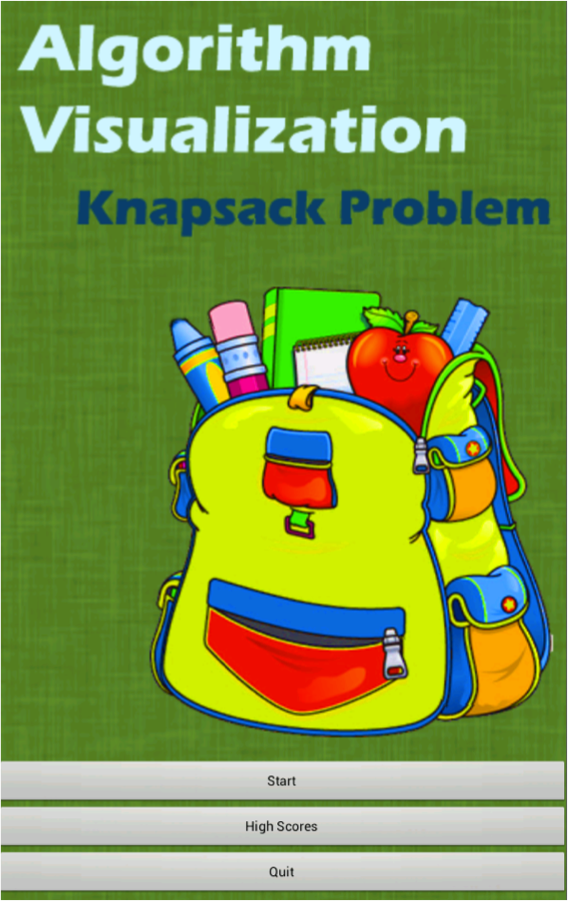
\includegraphics[scale=0.65]{splash_screen.png}
\caption{Startup splash screen for the knapsack problem}
\end{figure}

\subsection{High Scores}

The High Scores screen (Figure 2) displayes the best time for each level
(configured in an accompanying \texttt{.xml} file in the source code (see
Technical Documentation in Section 2).  The 'Reset High Score' button can be
used to clear the high score values for all levels, and the 'Return' button
takes the user back to the main menu.

\begin{figure}[h]
\centering
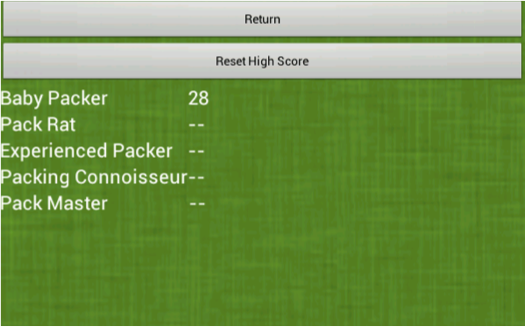
\includegraphics[scale=0.65]{high_scores.png}
\caption{High Scores screen}
\end{figure}

\subsection{Gameplay}

Upon beginning a game, a dialog (Figure 3) is displayed that allows the user to 
begin the game, which starts the timer that runs until the user submits the
attempted solution to the problem.

\begin{figure}[h]
\centering
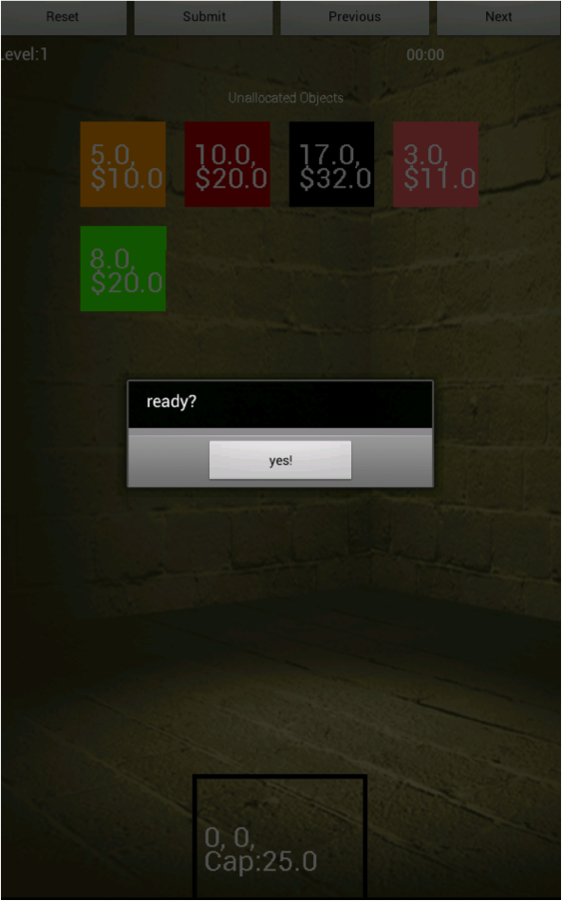
\includegraphics[scale=0.65]{level_start.png}
\caption{"Ready?" dialog at the beginning of each level}
\end{figure}

Each level in the game includes a series of objects, displayed at the top of the
screen, with associated weights and values.  At the bottom of the screen is a
series of one, two, or three bins, each with a certain weight capacity, as well
as the total value of the objects inside.

The object of the game is to touch and drag the objects into the bin(s) such
that the total value of the objects in the bins is maximized, without exceeding
the weight capacity of each bin.  As objects are added to the bins, the bin
will slowly fill to graphically show the remaining capacity of the bin.  See
Figure 4 for the basic layout of the game.

\begin{figure}[h]
\centering
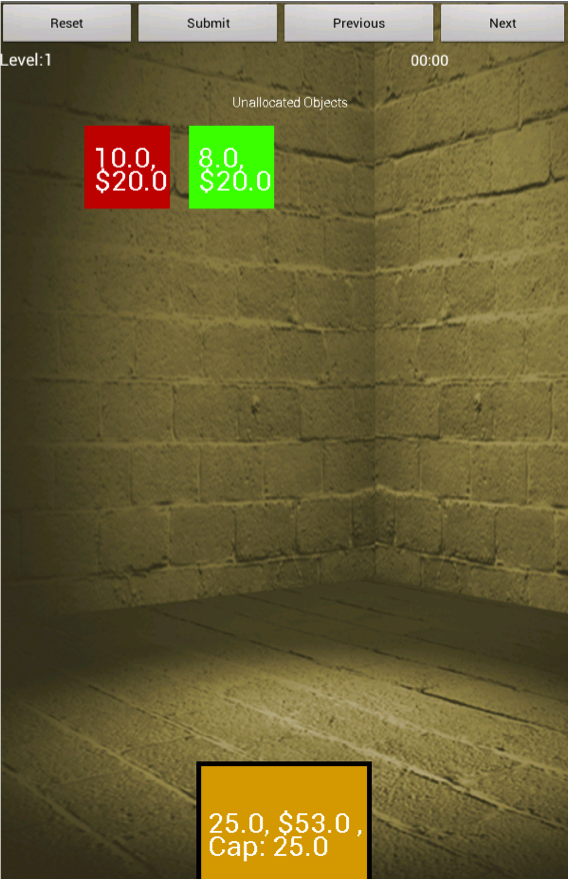
\includegraphics[scale=0.65]{gameplay.png}
\caption{Basic layout of gameplay}
\end{figure}

When the number of objects is large, left and right arrow buttons will allow the
user to scroll through a paginated list of objects.  The user may also touch the
bins to expand a page that displays the objects inside that bin (Figure 5).
From here, the objects can be dragged out of the bin entirely, or directly into
a different bin.  Touching the small 'X' in the upper right-hand corner of the
screen will allow the user to return to the page of unallocated objects.

\begin{figure}[h]
\centering
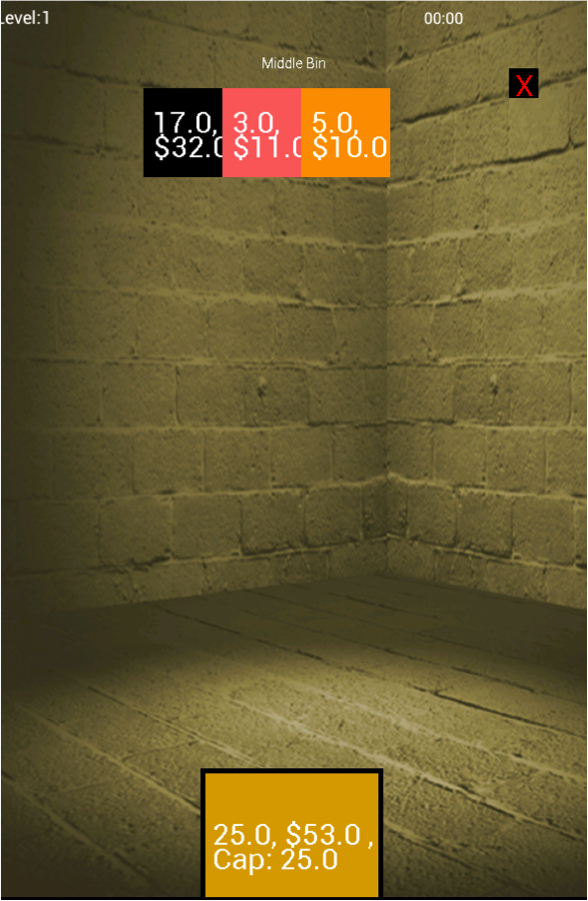
\includegraphics[scale=0.65]{inside_bin.png}
\caption{Objects inside bin}
\end{figure}

The user can submit the attempted allocation of objects by touching the 'Submit'
button at the top of the screen.  A dialog will appear indicating whether the
solution is optimal, and if not, the approximate percentage of the optimal
solution (i.e. optimal total value of objects in the bins) that our algorithm
generated.  Note that in the cases in which the number of bins is greater than
one, the bin-packing problem becomes NP-hard, therefore our algorithm only gives
an approximation to the actual optimal solution.  If the user finds a solution
greater than or equal to this approximation, it is considered correct.

\section{Technical Documentation}

This section gives a brief overview of the Java source code and its relation to
the GUI explained in Section 1, as well as the algorithm used to compute the
optimal solutions to the knapsack and bin-packing problems.  

\subsection{Basic dynamics of the Android GUI}

The three main views of the application as developed thus far (i.e. the main
menu, the high score screen, and the main gameplay screen) are governed by the
Java activity classes \texttt{AlgovizActivity.java},
\texttt{HighScoreActivity.java}, and \texttt{BinPackingActivity.java}
respectively.  These classes provide links between the three views, and contain
the main logic for computing the values associated with these views (e.g. the
values for the timer, the level numbers, etc.).

The class \texttt{BinPackingView.java} includes the vast majority of code
governing the graphics of the main gameplay view.  Objects are positioned on
the screen in this class, and the drag-and-drop capabilities are handled here.

\subsection{Supporting classes}

The code for the basic infrastructure of the application is contained in the
classes \texttt{BinObject.java}, \texttt{Bin.java}, and
\texttt{BinObjectPaginator.java}, which all extend \texttt{ShapeObject.java}.
These classes contain the values associated with each bin and object, the
details of how they are to be displayed, etc.  \texttt{BinObjectPaginator.java}
is used to display the objects in a bin, as well as to provide a means of
scrolling through objects when there are too many to be viewed on the screen
at once.

The \texttt{BinPackingProblemFactory.java} class is used to read in problem
configurations from a provided \texttt{.xml} file and parse the file as to 
extract the necessary values to be associated with the bins and objects.  It
also contains the Java implementation of the algorithm used to optimally
solve the problems (explained below).  The class \texttt{Scoreboard.java}
is used to manage the mechanics of high score storage.

There are also JUnit test cases written for much of the code, included
in the project repository along with the rest of the code.

\subsection{Bin-packing algorithm}

With only one bin involved, the bin-packing scenario represents an instance of
the knapsack problem. To calculate the optimal solution for the one-bin
scenario, we thus implemented the dynamic programming knapsack algorithm. We
used the algorithm's solution to check against the user's total "packed-in"
value, which allowed us to determine whether the user had reached the problem's
true optimal solution.

Scenarios with more than one bin represent instances of the bin-packing problem
(which is NP-hard). Here we could have implemented a brute-force approach for
calculating the optimal solution. However, since we allow app managers to define
an unbounded number of bin objects within problems.xml, the brute-force
algorithm's runtime could have quickly escalated to the point of slowing down
the app, which could have damaged user experience in the process. Thus, instead
of implementing a brute-force approach, we used heuristics to calculate an
approximate optimal solution. We based our approach around the knapsack
algorithm, which brought our solution's time complexity down to acceptable
levels.

To calculate the approximate solution we first made a copy of the set of all bin
objects -- call this set of objects $O'$. We then calculated the knapsack
solution for a single one of the bins. After calculating the solution, we
removed each object that the knapsack algorithm had used from $O'$. We then
repeated the knapsack algorithm for each of the bins, using $O'$ as the input,
and removing the set of bin objects that new calculation had used from the set
$O'$. Our approximation approach allows the app to run without any noticeable
performance penalties.

Finally, while the approximation algorithm's optimal solution was not
necessarily the exact optimal solution, we often found that the figure was high
enough to make each level challenging.

\subsection{Further information}

For further information, please contact the project group members at the email
addresses listed on the title page of this document.

\end{document}





